%%%%%%%%%%%%%%%%%%%%
%%% Document
%%%%%%%%%%%%%%%%%%%%
\documentclass[pdftex, a4paper,11pt, twoside, ngerman]{report}
% \documentclass[11pt,xcolor=dvipsnames]{beamer}

% für deutsche zeichen äüö ohne kile auto-ersetzen
% \usepackage[utf8x]{inputenc}

% kile auto-ersetzen: einstellungen->latex:general-> hacken bei special 
% characters
% \usepackage[ansinew]{inputenc}
% \usepackage[UKenglish]{babel}          %Englisch
\usepackage[ngerman]{babel}          %Deutsch
\usepackage{siunitx}


%%%%%%%%%%
%%% Geometry
%%%%%%%%%%
% \usepackage{showframe}
\usepackage[scale=0.8, hmarginratio=4:2]{geometry}
  \geometry{textheight=1.05\textheight, textwidth=.95\textwidth,
            marginparwidth=25 pt}



%%%%%%%%%%
%%% Packages (aus header datei)
%%%%%%%%%%
\IfFileExists{header_TobiasBrauell-DOCUMENT.tex}{
    % Copyright © 2014 Tobias Brauell <tobiasbrauell@gmail.com>

% This is my general purpose LaTeX header file for writing German documents.
% Ideally, you include this using a simple ``\input{header.tex}`` in your main
% document and start with ``\title`` and ``\begin{document}`` afterwards.

% If you need to add additional packages, I recommend not doing this in this
% file, but in your main document. That way, you can just drop in a new
% ``header.tex`` and get all the new commands without having to merge manually.

%%%%%%%%%%%%%%%%%%%%%%%%%%%%%
%%% Locale, date
%%%%%%%%%%%%%%%%%%%%%%%%%%%%%
\usepackage[UKenglish]{isodate}



%%%%%%%%%%%%%%%%%%%%%%%%%%%%%
%%% Margins and other spacing
%%%%%%%%%%%%%%%%%%%%%%%%%%%%%
\usepackage[activate]{pdfcprot}
% \usepackage[parfill]{parskip}
\usepackage{setspace}
  \setlength{\columnsep}{2 cm}
  \setlength{\parindent}{0 pt}


%%%%%%%%%%%%%%%%%%%%%%%%%%%%%
%%% Input encoding
%%%%%%%%%%%%%%%%%%%%%%%%%%%%%
\usepackage[T1]{fontenc}
\usepackage[utf8x]{inputenc}



%%%%%%%%%%%%%%%%%%%%%%%%%%%%%
%%% Indexing
%%%%%%%%%%%%%%%%%%%%%%%%%%%%%
\usepackage{makeidx}
  \makeindex



%%%%%%%%%%%%%%%%%%%%%%%%%%%%%
%%% Blindtext
%%%%%%%%%%%%%%%%%%%%%%%%%%%%%
\usepackage{blindtext}


%%%%%%%%%%%%%%%%%%%%%%%%%%%%%
%%% Global Counter
%%%%%%%%%%%%%%%%%%%%%%%%%%%%%



%%%%%%%%%%%%%%%%%%%%%%%%%%%%%
%%% Geometry
%%%%%%%%%%%%%%%%%%%%%%%%%%%%%
\usepackage{layout}
% \usepackage[scale=0.8]{geometry}
%   \geometry{textheight=1.05\textheight, marginparwidth=50 pt}

% \usepackage{multirow}
% \usepackage{dcolumn}



%%%%%%%%%%%%%%%%%%%%%%%%%%%%%
%%% Pagestyle
%%%%%%%%%%%%%%%%%%%%%%%%%%%%%
% \usepackage{fancyhdr}
% \usepackage{microtype} 

% \pagestyle{fancy}



%%%%%%%%%%%%%%%%%%%%%%%%%%%%%
%%% Fonts/Colors
%%%%%%%%%%%%%%%%%%%%%%%%%%%%%
\usepackage{lmodern}
\usepackage{xcolor}
% This replaces all fonts with Bitstream Charter, Bitstream Vera Sans and
% Bitstream Vera Mono. Math will be rendered in Charter.
% \usepackage[charter, greekuppercase=italicized]{mathdesign}
% \usepackage{beramono}
% \usepackage{berasans}

% Bold, sans-serif tensors. This fragment is taken from “egreg” from
% http://tex.stackexchange.com/a/82747/8945 and licensed under `CC-BY-SA
% <https://creativecommons.org/licenses/by-sa/3.0/>`_.
% \usepackage{bm}
%   \DeclareMathAlphabet{\mathsfit}{\encodingdefault}{\sfdefault}{m}{sl}
%   \SetMathAlphabet{\mathsfit}{bold}{\encodingdefault}{\sfdefault}{bx}{sl}
%   \newcommand{\tens}[1]{\bm{\mathsfit{#1}}}

% Bold vectors.
% \renewcommand{\vec}[1]{\boldsymbol{#1}}



%%%%%%%%%%%%%%%%%%%%%%%%%%%%%
%%% Code/Listings
%%%%%%%%%%%%%%%%%%%%%%%%%%%%%
\usepackage{listings}



%%%%%%%%%%%%%%%%%%%%%%%%%%%%%
%%% Enumerations
%%%%%%%%%%%%%%%%%%%%%%%%%%%%%
\usepackage{enumitem}
% \usepackage{paralist}


%%%%%%%%%%%%%%%%%%%%%%%%%%%%%
%%% Figures
%%%%%%%%%%%%%%%%%%%%%%%%%%%%%
% \usepackage[pdftex]{graphicx}
\usepackage{graphicx}
\usepackage{epsfig}
\usepackage{epstopdf}
\usepackage{subfigure}
\usepackage{wrapfig}
\makeatletter \newcommand\hyper@makecurrent[1]{} \makeatother
\usepackage{caption}
% \usepackage{subcaption}

\addto\captionsUKenglish{\renewcommand{\figurename}{Fig.}}
\addto\captionsngerman{\renewcommand{\figurename}{Abb.}}



%%%%%%%%%%%%%%%%%%%%%%%%%%%%%
%%% PDF Pages
%%%%%%%%%%%%%%%%%%%%%%%%%%%%%
\usepackage{pdfpages}



%%%%%%%%%%%%%%%%%%%%%%%%%%%%%
%%% Personal Graphics
%%%%%%%%%%%%%%%%%%%%%%%%%%%%%
\usepackage{tikz}
% \usepackage{tikz-3dplot}
  \usetikzlibrary{calc}
  \usetikzlibrary{decorations.markings}



%%%%%%%%%%%%%%%%%%%%%%%%%%%%%
%%% Math
%%%%%%%%%%%%%%%%%%%%%%%%%%%%%
\usepackage{amsmath}
\usepackage{amssymb}
\usepackage{mathtools}
\usepackage{dcolumn}
\usepackage{siunitx}
% \usepackage{feynmf}



%%%%%%%%%%%%%%%%%%%%%%%%%%%%%
%%% Referenzen
%%%%%%%%%%%%%%%%%%%%%%%%%%%%%
\usepackage{hyperref}
\usepackage{url}
% \usepackage{cleveref}%\label{abc}--\cref{abc} \Cref{abc[,def]}-und \crefrange{abc}{def}-bis
\usepackage[english]{cleveref}%\label{abc}--\cref{abc} \Cref{abc[,def]}-und \crefrange{abc}{def}-bis



%%%%%%%%%%%%%%%%%%%%%%%%%%%%%
%%% Table's
%%%%%%%%%%%%%%%%%%%%%%%%%%%%%
\usepackage{rotating}
\usepackage{longtable}
\usepackage{multirow}
\usepackage{tabularx}
  \newcolumntype{L}[1]{>{\raggedright\arraybackslash}p{#1}} % linksbündig mit Breitenangabe
  \newcolumntype{C}[1]{>{\centering\arraybackslash}p{#1}} % zentriert mit Breitenangabe
  \newcolumntype{R}[1]{>{\raggedleft\arraybackslash}p{#1}} % rechtsbündig mit Breitenangabe



%%%%%%%%%%%%%%%%%%%%%%%%%%%%%
%%% Todo's
%%%%%%%%%%%%%%%%%%%%%%%%%%%%%
% \usepackage{xkeyval}
\usepackage{todonotes} %\todo{text} oder \todo[inline]{text}
%   \presetkeys{todonotes}{inline}{}
%   \let\todox\todo
%   \renewcommand\todo{1}{\todox[inline]{#1}}


%%%%%%%%%%%%%%%%%%%%%%%%%%%%%%%%%%%%%%%%%%%%%%%%%%%%%%%%%%
%%% Settings
%%%%%%%%%%%%%%%%%%%%%%%%%%%%%%%%%%%%%%%%%%%%%%%%%%%%%%%%%%
\usepackage{cancel}

\newcommand{\HRule}{\rule{\linewidth}{0.5mm}}



%%%%%%%%%%%%%%%%%%%%%%%%%%%%%
%%% Theme
%%%%%%%%%%%%%%%%%%%%%%%%%%%%%



%%%%%%%%%%%%%%%%%%%%%%%%%%%%%
%%% header
%%%%%%%%%%%%%%%%%%%%%%%%%%%%%
% \lhead{text}
% \chead{text}
% \rhead{text}



%%%%%%%%%%%%%%%%%%%%%%%%%%%%%
%%% footer
%%%%%%%%%%%%%%%%%%%%%%%%%%%%%
%%% Tobias Brauell       	Versuch....		Ruth Jacobs
% \renewcommand\footrulewidth{.4pt}
% \lfoot{\scriptsize Ruth Jacobs - Tobias Brauell \\ {\ \ \ \ \ \ \ \ \ \ } Gruppe $\alpha 9$} 
% \cfoot{\thepage\ / \ \pageref{LastPage}}
% \rfoot{\scriptsize Versuch 518: Höhenstrahlung \\ Tutor: Christoph Krieger {\ \ \ } } 



%%%%%%%%%%%%%%%%%%%%%%%%%%%%%
%%% Title Page
%%%%%%%%%%%%%%%%%%%%%%%%%%%%%
% \title[ITER { } International Thermonuclear Experimental Reactor]{\huge{\bf{ITER}} \\ \large{\bf{International Thermonuclear Experimental Reactor}}}
% \author[T. Brauell]{Tobias Brauell}
% \institute{Universität Bonn}
% 
% \date{09.~Dez.~2013}
% \logo{\includegraphics[width=.15\textwidth]{Figures/toplogo.png}}


}{
    % Copyright © 2014 Tobias Brauell <tobiasbrauell@gmail.com>

% This is my general purpose LaTeX header file for writing German documents.
% Ideally, you include this using a simple ``\input{header.tex}`` in your main
% document and start with ``\title`` and ``\begin{document}`` afterwards.

% If you need to add additional packages, I recommend not doing this in this
% file, but in your main document. That way, you can just drop in a new
% ``header.tex`` and get all the new commands without having to merge manually.

%%%%%%%%%%%%%%%%%%%%%%%%%%%%%
%%% Locale, date
%%%%%%%%%%%%%%%%%%%%%%%%%%%%%
\usepackage[UKenglish]{isodate}



%%%%%%%%%%%%%%%%%%%%%%%%%%%%%
%%% Margins and other spacing
%%%%%%%%%%%%%%%%%%%%%%%%%%%%%
\usepackage[activate]{pdfcprot}
% \usepackage[parfill]{parskip}
\usepackage{setspace}
  \setlength{\columnsep}{2 cm}
  \setlength{\parindent}{0 pt}


%%%%%%%%%%%%%%%%%%%%%%%%%%%%%
%%% Input encoding
%%%%%%%%%%%%%%%%%%%%%%%%%%%%%
\usepackage[T1]{fontenc}
\usepackage[utf8x]{inputenc}



%%%%%%%%%%%%%%%%%%%%%%%%%%%%%
%%% Indexing
%%%%%%%%%%%%%%%%%%%%%%%%%%%%%
\usepackage{makeidx}
  \makeindex



%%%%%%%%%%%%%%%%%%%%%%%%%%%%%
%%% Blindtext
%%%%%%%%%%%%%%%%%%%%%%%%%%%%%
\usepackage{blindtext}


%%%%%%%%%%%%%%%%%%%%%%%%%%%%%
%%% Global Counter
%%%%%%%%%%%%%%%%%%%%%%%%%%%%%



%%%%%%%%%%%%%%%%%%%%%%%%%%%%%
%%% Geometry
%%%%%%%%%%%%%%%%%%%%%%%%%%%%%
\usepackage{layout}
% \usepackage[scale=0.8]{geometry}
%   \geometry{textheight=1.05\textheight, marginparwidth=50 pt}

% \usepackage{multirow}
% \usepackage{dcolumn}



%%%%%%%%%%%%%%%%%%%%%%%%%%%%%
%%% Pagestyle
%%%%%%%%%%%%%%%%%%%%%%%%%%%%%
% \usepackage{fancyhdr}
% \usepackage{microtype} 

% \pagestyle{fancy}



%%%%%%%%%%%%%%%%%%%%%%%%%%%%%
%%% Fonts/Colors
%%%%%%%%%%%%%%%%%%%%%%%%%%%%%
\usepackage{lmodern}
\usepackage{xcolor}
% This replaces all fonts with Bitstream Charter, Bitstream Vera Sans and
% Bitstream Vera Mono. Math will be rendered in Charter.
% \usepackage[charter, greekuppercase=italicized]{mathdesign}
% \usepackage{beramono}
% \usepackage{berasans}

% Bold, sans-serif tensors. This fragment is taken from “egreg” from
% http://tex.stackexchange.com/a/82747/8945 and licensed under `CC-BY-SA
% <https://creativecommons.org/licenses/by-sa/3.0/>`_.
% \usepackage{bm}
%   \DeclareMathAlphabet{\mathsfit}{\encodingdefault}{\sfdefault}{m}{sl}
%   \SetMathAlphabet{\mathsfit}{bold}{\encodingdefault}{\sfdefault}{bx}{sl}
%   \newcommand{\tens}[1]{\bm{\mathsfit{#1}}}

% Bold vectors.
% \renewcommand{\vec}[1]{\boldsymbol{#1}}



%%%%%%%%%%%%%%%%%%%%%%%%%%%%%
%%% Code/Listings
%%%%%%%%%%%%%%%%%%%%%%%%%%%%%
\usepackage{listings}



%%%%%%%%%%%%%%%%%%%%%%%%%%%%%
%%% Enumerations
%%%%%%%%%%%%%%%%%%%%%%%%%%%%%
\usepackage{enumitem}
% \usepackage{paralist}


%%%%%%%%%%%%%%%%%%%%%%%%%%%%%
%%% Figures
%%%%%%%%%%%%%%%%%%%%%%%%%%%%%
% \usepackage[pdftex]{graphicx}
\usepackage{graphicx}
\usepackage{epsfig}
\usepackage{epstopdf}
\usepackage{subfigure}
\usepackage{wrapfig}
\makeatletter \newcommand\hyper@makecurrent[1]{} \makeatother
\usepackage{caption}
% \usepackage{subcaption}

\addto\captionsUKenglish{\renewcommand{\figurename}{Fig.}}
\addto\captionsngerman{\renewcommand{\figurename}{Abb.}}



%%%%%%%%%%%%%%%%%%%%%%%%%%%%%
%%% PDF Pages
%%%%%%%%%%%%%%%%%%%%%%%%%%%%%
\usepackage{pdfpages}



%%%%%%%%%%%%%%%%%%%%%%%%%%%%%
%%% Personal Graphics
%%%%%%%%%%%%%%%%%%%%%%%%%%%%%
\usepackage{tikz}
% \usepackage{tikz-3dplot}
  \usetikzlibrary{calc}
  \usetikzlibrary{decorations.markings}



%%%%%%%%%%%%%%%%%%%%%%%%%%%%%
%%% Math
%%%%%%%%%%%%%%%%%%%%%%%%%%%%%
\usepackage{amsmath}
\usepackage{amssymb}
\usepackage{mathtools}
\usepackage{dcolumn}
\usepackage{siunitx}
% \usepackage{feynmf}



%%%%%%%%%%%%%%%%%%%%%%%%%%%%%
%%% Referenzen
%%%%%%%%%%%%%%%%%%%%%%%%%%%%%
\usepackage{hyperref}
\usepackage{url}
% \usepackage{cleveref}%\label{abc}--\cref{abc} \Cref{abc[,def]}-und \crefrange{abc}{def}-bis
\usepackage[english]{cleveref}%\label{abc}--\cref{abc} \Cref{abc[,def]}-und \crefrange{abc}{def}-bis



%%%%%%%%%%%%%%%%%%%%%%%%%%%%%
%%% Table's
%%%%%%%%%%%%%%%%%%%%%%%%%%%%%
\usepackage{rotating}
\usepackage{longtable}
\usepackage{multirow}
\usepackage{tabularx}
  \newcolumntype{L}[1]{>{\raggedright\arraybackslash}p{#1}} % linksbündig mit Breitenangabe
  \newcolumntype{C}[1]{>{\centering\arraybackslash}p{#1}} % zentriert mit Breitenangabe
  \newcolumntype{R}[1]{>{\raggedleft\arraybackslash}p{#1}} % rechtsbündig mit Breitenangabe



%%%%%%%%%%%%%%%%%%%%%%%%%%%%%
%%% Todo's
%%%%%%%%%%%%%%%%%%%%%%%%%%%%%
% \usepackage{xkeyval}
\usepackage{todonotes} %\todo{text} oder \todo[inline]{text}
%   \presetkeys{todonotes}{inline}{}
%   \let\todox\todo
%   \renewcommand\todo{1}{\todox[inline]{#1}}


%%%%%%%%%%%%%%%%%%%%%%%%%%%%%%%%%%%%%%%%%%%%%%%%%%%%%%%%%%
%%% Settings
%%%%%%%%%%%%%%%%%%%%%%%%%%%%%%%%%%%%%%%%%%%%%%%%%%%%%%%%%%
\usepackage{cancel}

\newcommand{\HRule}{\rule{\linewidth}{0.5mm}}



%%%%%%%%%%%%%%%%%%%%%%%%%%%%%
%%% Theme
%%%%%%%%%%%%%%%%%%%%%%%%%%%%%



%%%%%%%%%%%%%%%%%%%%%%%%%%%%%
%%% header
%%%%%%%%%%%%%%%%%%%%%%%%%%%%%
% \lhead{text}
% \chead{text}
% \rhead{text}



%%%%%%%%%%%%%%%%%%%%%%%%%%%%%
%%% footer
%%%%%%%%%%%%%%%%%%%%%%%%%%%%%
%%% Tobias Brauell       	Versuch....		Ruth Jacobs
% \renewcommand\footrulewidth{.4pt}
% \lfoot{\scriptsize Ruth Jacobs - Tobias Brauell \\ {\ \ \ \ \ \ \ \ \ \ } Gruppe $\alpha 9$} 
% \cfoot{\thepage\ / \ \pageref{LastPage}}
% \rfoot{\scriptsize Versuch 518: Höhenstrahlung \\ Tutor: Christoph Krieger {\ \ \ } } 



%%%%%%%%%%%%%%%%%%%%%%%%%%%%%
%%% Title Page
%%%%%%%%%%%%%%%%%%%%%%%%%%%%%
% \title[ITER { } International Thermonuclear Experimental Reactor]{\huge{\bf{ITER}} \\ \large{\bf{International Thermonuclear Experimental Reactor}}}
% \author[T. Brauell]{Tobias Brauell}
% \institute{Universität Bonn}
% 
% \date{09.~Dez.~2013}
% \logo{\includegraphics[width=.15\textwidth]{Figures/toplogo.png}}


}



%%%%%%%%%%
%%%%%%%%%%
%%%%%%%%%%
\begin{document}
%   \layout
  %%%%%%%%%%%%%%%%%%%%%%%%%%%%%%%%%%%%%%%%%%%%%%%%%%%%%%%%%%
%%% Title Page - Bachelor Thesis
%%%%%%%%%%%%%%%%%%%%%%%%%%%%%%%%%%%%%%%%%%%%%%%%%%%%%%%%%%
\begin{titlepage}
  \thispagestyle{empty}
  \begin{center}

    % Upper part of the page. The '~' is needed because \\
    % only works if a paragraph has started.
%     \includegraphics[width=0.15\textwidth]{./logo}~\\[1cm]
    \begin{minipage}{0.5\textwidth}
      \begin{flushleft}
	
\includegraphics[width=.5\textwidth]{Figures/logoUNI.png}
      \end{flushleft}
    \end{minipage}%
    \begin{minipage}{0.5\textwidth}
      \begin{flushright}
	
\includegraphics[width=.5\textwidth]{Figures/logoPI.png}
      \end{flushright}
    \end{minipage}
    
    \vspace{25 pt}
    
    \textsc{\LARGE Rheinische Friedrich-Wilhelms-Universität Bonn}\\[1.5 cm]
    
    \vspace{50 pt}
    
    \textsc{\Large Praktikum 4 - Atome und Moleküle}\\[0.5 cm]

    % Title
    \HRule \\[0.4 cm]
    { \huge \bfseries Versuch 402 - Quantelung von Energie \\[0.4 cm] }

    \HRule \\[1.5 cm]

    % Author and supervisor
    \noindent
    \begin{minipage}{0.4\textwidth}
      \begin{flushleft} \large
	\emph{Authors:}\\
	Tobias \textsc{Brauell}\\
	Frederike \textsc{Schrödel}
      \end{flushleft}
    \end{minipage}%
    \begin{minipage}{0.4\textwidth}
      \begin{flushright} \large
	\emph{Supervisor:} \\
	Dennis \textsc{Proft}
      \end{flushright}
    \end{minipage}

    \vfill

    % Bottom of the page
    \HRule \\[0.4 cm]
    {\large \today}

  \end{center}
\end{titlepage}
%   \setcounter{page}{2}
  
  \begin{chapter}*{Abstract}
    Ziel des Versuchs ist es den Zusammenhang zwischen Energie und Frequenz des
    Lichts zu bestimmen. Hierzu wird die Quantelung der Energie sowohl durch 
    den Photoeffekt, als auch durch die Messung der Balmerserie von 
    Wasserstoff und Deuterium bestimmt. Somit erhalten wir Werte für das 
    Plancksche Wirkungsquantum die im Anschluss verglichen werden. 
  \end{chapter}
  
  \tableofcontents
  
  
  
  %%%%%%%%%%%%%%%%%%%%
  %%%%%%%%%%%%%%%%%%%%
  %%%%%%%%%%%%%%%%%%%%
  \begin{chapter}{Theorie des Versuchs}
    \label{chp:Theorie}
    Für die Durchführung eines jeden Labor-Versuches ist es wichtig bereits vor
    dem eigentlichen Beginn des Versuches die benötigte Theorie zu kennen und 
    zu verstehen. Daher werden hier zu aller erst die beteiligten 
    theoretischen und physikalischen Grundlagen erklärt.
    
    
    
    %%%%%%%%%%%%%%%%%%%%%%%%%%%%%%
    %%%%%%%%%%%%%%%%%%%%%%%%%%%%%%
    %%%%%%%%%%%%%%%%%%%%%%%%%%%%%%
    \begin{section}{Photoelektrische Bestimmung des Planckschen Wirkungsquant}
      \label{chp:TheoriePhotoelektrischesWirkungsquantum}
      
      
      
      %%%%%%%%%%%%%%%%%%%%%%%%%%%%%%%%%%%%%%%%
      %%%%%%%%%%%%%%%%%%%%%%%%%%%%%%%%%%%%%%%%
      %%%%%%%%%%%%%%%%%%%%%%%%%%%%%%%%%%%%%%%%
      \begin{subsection}{Photoeffekt}
        \label{chp:TheoriePhotoelektrischesWirkungsquantumPhotoeffekt}
%         Unter dem Photoeffekt versteht man den klassisch betrachtet 
%         verblüffenden Effekt, dass die Energie eines Elektrons, welches durch 
%         ein Photon aus einer Photokathode ausgelöst wird, nur von der 
%         Frequenz des Lichts, aber nicht von der Intensität abhängt. 
        Der Photoeffekt, oder auch Photoelektrischer Effekt genannt, bezeichnet
        eine physikalische Eigenschaft der Atomhülle mithilfe derer die
        Energie eines Hüllenelektrons beeinflusst werden kann. Dabei
        wechselwirkt ein energiereiches Photon mit einem Hüllenelektron und
        übergibt diesem seinem gesamten Impuls und ändert somit die Energie
        des Elektrons. Die Energie des Photons ist nach Einstein mit der
        \cref{eq:EnergiePhoton} gegeben.
        \begin{equation}
          \label{eq:EnergiePhoton}
          E=h\nu=\frac{hc}{\lambda}
        \end{equation}
        Daraus geht also hervor, dass die Energie antiproportional zur 
        Wellenlänge des Photons ist. Abhängig von der Energie des absorbierten 
        Photons reagiert das Elektron mit einer Änderung seiner Bahn um den 
        Atomkern. Das nun angeregte Elektron wechselt in eine höhere Schale. 
        Erhält das Elektron genügend Energie, so kann es komplett aus dem Atom 
        entfernt werden. Diese Energie wird als \textit{Ionisierungsenergie} 
        bezeichnet.
        
        \todo[inline]{Reicht das hier schon? vielleicht noch etwas zu 
            Absorptionslinien und Emissionslinien}
        
        \begin{figure}[htbp]
          \centering
          \begin{minipage}{0.48\textwidth}
            \centering
            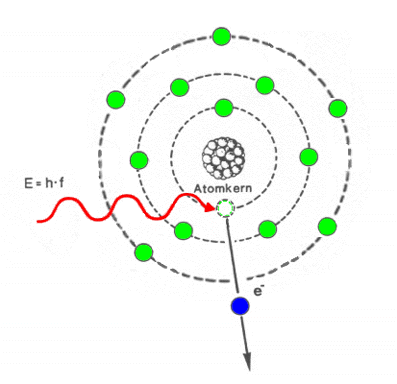
\includegraphics[width=.9\textwidth]{Figures/photoeffekt.png}
            \caption{Schematische Darstellung der Wirkungsweise des 
                Photoeffekts.\cite{bib:Photoeffekt}}
            \label{fig:Photoeffekt}
          \end{minipage}\quad
          \begin{minipage}{0.48\textwidth}
            \centering
            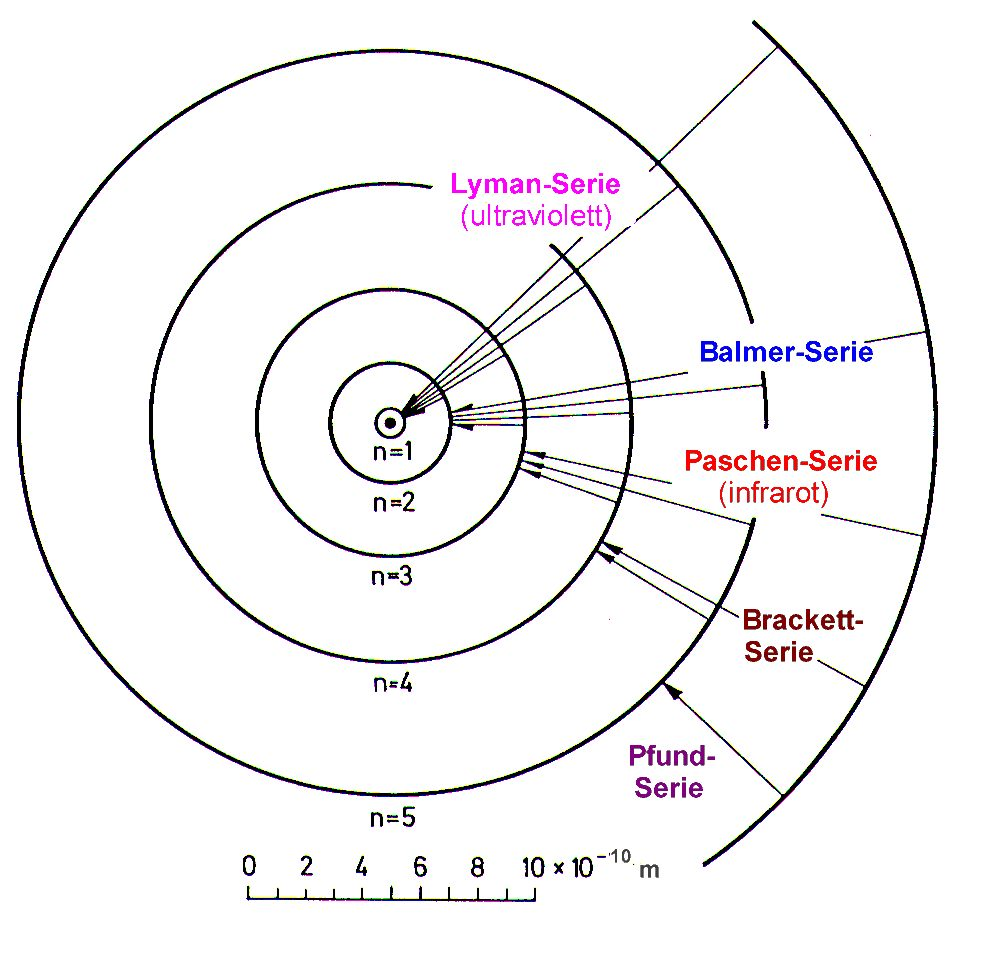
\includegraphics[width=.9\textwidth]
                {Figures/BohrschesAtommodellSerien.png}
            \caption{Bohrsches Atommodell zusammen mit den Übergangsserien.
                \cite{bib:BohrschesAtommodellSerien}}
            \label{fig:BohrschesAtommodellSerien}
          \end{minipage}
        \end{figure}
        
      \end{subsection}
      %%%%%%%%%%%%%%%%%%%%%%%%%%%%%%%%%%%%%%%%
      
      
      
      %%%%%%%%%%%%%%%%%%%%%%%%%%%%%%%%%%%%%%%%
      %%%%%%%%%%%%%%%%%%%%%%%%%%%%%%%%%%%%%%%%
      %%%%%%%%%%%%%%%%%%%%%%%%%%%%%%%%%%%%%%%%
      \begin{subsection}{Photozelle}
        \label{chp:TheoriePhotoelektrischesWirkungsquantumPhotozelle}
        In diesem Versuch wird der Photoeffekt u.A. dafür genutzt um Elektronen
        aus einer Metallplatte heraus zu lösen. Dabei trifft Das Licht einer 
        Quecksilberdampflampe mit einer ionisierenden Wellenlänge auf eine 
        negativ geladene Metallplatte. Um ein Elektron aus der Oberfläche zu 
        lösen muss die spezifische Austrittsarbeit des verwendeten Metalls 
        erreicht werden. Aus der Austrittsarbeit ergibt sich mithilfe von 
        \cref{eq:Grenzfrequenz} die sog. \textit{Grenzfrequenz}.
        \begin{equation}
          \label{eq:Grenzfrequenz}
          \nu_{0}=\frac{W_{A}}{h}
        \end{equation}
        Die ausgelösten Elektronen können anschließend in der Photozelle
        detektiert werden. Aufgebaut ist die Photozelle aus einem evakuierten 
        Gehäuse in dem eine Metallplatte als Kathode angebracht ist. Auf der 
        gegenüber liegenden Seite innerhalb des Gehäuses ist ein dünner 
        Ringdraht als Anode angeschlossen. An Anode und Kathode kann nun eine 
        Spannung angelegt werden um die ausgelösten Elektronen einem Potential 
        auszusetzen. Wird nun Spannung erhöht, werden die Elektronen zur Anode 
        hin beschleunigt und können als Strom mit einem Amperemeter gemessen 
        werden. Wird die Spannung umgepolt, so werden die Elektronen zurück 
        auf die Metallplatte beschleunigt und der Anodenstrom verringert sich. 
        So kann man die kinetische Energie der ausgelösten Elektronen finden 
        indem man die Grenzspannung bestimmt, bei der kein Anodenstrom mehr 
        gemessen werden kann. Die maximale kinetische Energie ergibt sich dann 
        aus der Differenz der Energie des Photons und der Austrittsarbeit mit 
        \cref{eq:Ekin}.
        \begin{equation}
          \label{eq:Ekin}
          E_{kin}=eU_{0}=h\nu-W_{A}
        \end{equation}
        
        \begin{figure}[b]
          \begin{center}
            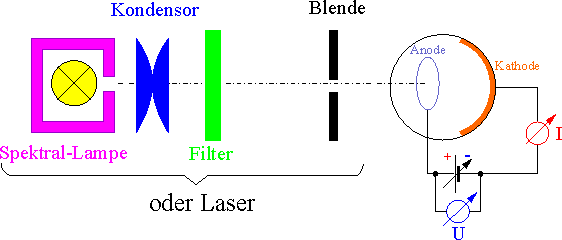
\includegraphics[width=.8\textwidth]
                {Figures/photozelle_mit_aufbau.png}
            \caption{Schematischer Aufbau einer Photozelle.
                \cite{bib:PhotozelleAufbau}}
            \label{fig:PhotozelleAufbau}
          \end{center}
        \end{figure}
        
        Um möglichst genaue Messwerte zu erhalten werden Anode und Kathode aus
        Materialien mit unterschiedlichen Ionisierungsenergien verwendet. 
        Dadurch kann es vermieden werden, dass der Anodenstrom durch 
        Elektronen verfälscht wird, die aus der Anode selbst gelöst wurden. 
        Die Verbindung unterschiedlicher Materialien bringt allerdings den 
        Nachteil mit sich, dass zwischen ihnen ein sog. 
        \textit{Kontaktpotential} entsteht. Dieses Kontaktpotential entsteht,
        da sich die Potentiale (oder Fermi-Niveaus) beider Kontakte im 
        Gleichgewicht befinden müssen. Daher kommt zu dieser Gleichung noch 
        eine Korrektur für das Kontaktpotential zwischen den Materialien hinzu
        die in \cref{eq:KontaktpotentialKorrektur} gegeben ist.
        \begin{equation}
          \label{eq:KontaktpotentialKorrektur}
          W_{K}^{12}=\left|W_{A}^{1}-W_{A}^{2}\right|
        \end{equation}
        Daraus ergibt sich somit die Kontaktpotential korrigierte Formel für
        die kinetische Energie \cref{eq:EkinKontaktpotential}.
        \begin{equation}
          \label{eq:EkinKontaktpotential}
          E_{kin}=eU_{0}-W_{K}=h\nu-W_{A}-W_{K}
        \end{equation}
        
        \todo[inline]{Sind alle Formel richtig?}
        
      \end{subsection}
      %%%%%%%%%%%%%%%%%%%%%%%%%%%%%%%%%%%%%%%%
      
    \end{section}
    %%%%%%%%%%%%%%%%%%%%%%%%%%%%%%
    
    
    
    %%%%%%%%%%%%%%%%%%%%%%%%%%%%%%
    %%%%%%%%%%%%%%%%%%%%%%%%%%%%%%
    %%%%%%%%%%%%%%%%%%%%%%%%%%%%%%
    \begin{section}{Bohrsches Atommodell und Balmer-Serie}
      \label{chp:TheorieBohrBalmerSerie}
      
      
      
      %%%%%%%%%%%%%%%%%%%%%%%%%%%%%%%%%%%%%%%%
      %%%%%%%%%%%%%%%%%%%%%%%%%%%%%%%%%%%%%%%%
      %%%%%%%%%%%%%%%%%%%%%%%%%%%%%%%%%%%%%%%%
      \begin{subsection}{Aufbau des Borschen Atoms}
        \label{chp:TheorieBohrBalmerSerieAufbauAtomhuelle}
        Das Bohrsche Atommodell ist das wohl bekannteste Atommodell. Für sein
        Modell postulierte Bohr $1913$ die folgenden drei Postulate.
        \begin{enumerate}
          \item Elektronen umkreisen den Atomkern auf festen Bahnen.
          \item Das Elektron kann den Kern nur stabil und ohne 
              Energieabstrahlung auf bestimmten, diskreten Bahnen mit festen 
              Energien umkreisen.
          \item Elektronen können ihre Energie nur durch Emission oder 
              Absorption elektromagnetischer Strahlung ändern.
        \end{enumerate}
        Die Radien der diskreten Bahnen dieser Postulate sind mit 
        \cref{eq:Bohrradius} und deren Energien mit 
        \cref{eq:BohrradiusEnergien}.
        \newline
        \begin{minipage}{.48\textwidth}
          \begin{equation}
            \label{eq:Bohrradius}
            r_{n}=\frac{n^{2}}{Z}a_{0}=\frac{n^{2}h^{2}\epsilon_{0}}
                {\pi\nu Ze^{2}}
          \end{equation}
        \end{minipage}
        \begin{minipage}{.48\textwidth}
          \begin{equation}
            \label{eq:BohrradiusEnergien}
            E_{n}=-R_{y}\frac{Z^{2}}{n^{2}}
          \end{equation}
        \end{minipage}
        
        \todo[inline]{Hier muss noch was weiter gemacht werden. vielleicht
        etwas zu bahnwechseln ueber Absorption und Emission.}
        
      \end{subsection}
      %%%%%%%%%%%%%%%%%%%%%%%%%%%%%%%%%%%%%%%%
      
      
      
      %%%%%%%%%%%%%%%%%%%%%%%%%%%%%%%%%%%%%%%%
      %%%%%%%%%%%%%%%%%%%%%%%%%%%%%%%%%%%%%%%%
      %%%%%%%%%%%%%%%%%%%%%%%%%%%%%%%%%%%%%%%%
      \begin{subsection}{Spektroskopie}
        \label{chp:TheorieBohrBalmerSerieSpektroskopie}
        Unter den Begriff Spektroskopie fasst man verschiedene Verfahren
        zusammen, Energie in ihr Spektrum zerlegen.
        Wir haben es hier mit der Spektroskopie an einem Refelktionsgitter zu
        tun.
        \begin{figure}[b]
          \begin{center}
            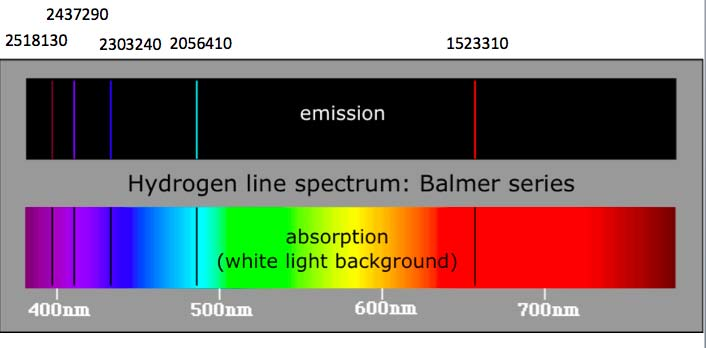
\includegraphics[width=.95\textwidth]
                {Figures/BalmerserieEmissionAbsorption.png}
            \caption{Emissions- und Absorptionslinien der Balmer Übergänge im 
                Wasserstoff Atom.
                \cite{bib:BalmerserieEmissionAbsorption}}
            \label{fig:BalmerserieEmissionAbsorption}
          \end{center}
        \end{figure}
        Zur späteren Bestimmung der Gitterkonstante $g$ nutzen wir die
        Gittergleichung:
        \begin{equation}
          \label{eq:Gittergleichung}
          g(\sin(\alpha)+\sin(\beta))=m\lambda
        \end{equation}
        
        \begin{figure}[htbp]
          \begin{center}
            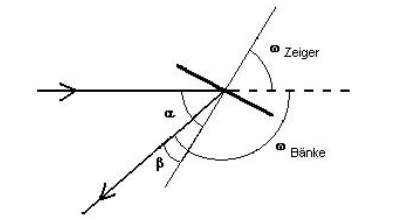
\includegraphics[width=.8\textwidth]{Figures/Gitteraufbau.png}
            \caption{Schematische Darstellung des Reflektionsgitteraufbaus.
                \cite{bib:LDDidactic}}
            \label{fig:Gitteraufbau}
          \end{center}
        \end{figure}
        
        Es werden die Emissionspektren der Quecksilberdampflampe und der Balmer
        Lampe hiermit sichtbar gemacht.
      
      \end{subsection}
      %%%%%%%%%%%%%%%%%%%%%%%%%%%%%%%%%%%%%%%%
      
      
      
      %%%%%%%%%%%%%%%%%%%%%%%%%%%%%%%%%%%%%%%%
      %%%%%%%%%%%%%%%%%%%%%%%%%%%%%%%%%%%%%%%%
      %%%%%%%%%%%%%%%%%%%%%%%%%%%%%%%%%%%%%%%%
      \begin{subsection}{Linienbreite}
        \label{chp:TheorieBohrBalmerSerieLinienbreite}
        Ein wichtiger Punkt bei der Spektroskopie ist die Linienbreite. Es gibt
        verschiedene Effekte, welche die Linienbreite beeinflussen. Die 
        natürliche Linienbreite, minimale Breite der Spektrallinie, tritt 
        sogar bei einem völlig isolierten Atom. Sie entsteht auf Grund der 
        endlichen Strahlungsdauer des Atoms. Hierdurch kommt es zu einer 
        Energie-Zeitunschärfe, in der Form einer Resonazkurve. Zusätzlich zu 
        der natürlichen Linienbreite gibt es die Dopplerverbreiterung, welche 
        durch die Summe  der Bewegung der einzelnen Teilchen in 
        unterschiedliche Raumrichtungen entsteht. Bei höheren Temperaturen 
        verstärkt sich dieser Effekt, durch die steigende mittlere 
        Geschwindigkeit der Teilchen. Die Stoßverbreiterung bewirkt bei 
        benachbarten Atomen eine Verschiebung der Energieniveaus. Durch Stöße 
        wird die Lebensdauer eines angeregten Zustandes verkürzt, sodass die 
        Energie unschärfer wird.
        
        \todo[inline]{formel}
        
      \end{subsection}
      %%%%%%%%%%%%%%%%%%%%%%%%%%%%%%%%%%%%%%%%
      
    \end{section}
    %%%%%%%%%%%%%%%%%%%%%%%%%%%%%%

  \end{chapter}
  %%%%%%%%%%%%%%%%%%%%
          
          
          
  %%%%%%%%%%%%%%%%%%%%
  %%%%%%%%%%%%%%%%%%%%
  %%%%%%%%%%%%%%%%%%%%
  \begin{chapter}{Erster Versuchsteil - Photoeffekt}
    \label{chp:Photoeffekt}
    
    
    
    %%%%%%%%%%%%%%%%%%%%%%%%%%%%%%
    %%%%%%%%%%%%%%%%%%%%%%%%%%%%%%
    %%%%%%%%%%%%%%%%%%%%%%%%%%%%%%
    \begin{section}{Aufbau und Justage}
      \label{chp:photoeffekt:sec:AufbauJustage}
      Wie in der Skizze zu sehen besteht der Aufbau aus einer Hg Lampe, einer
      Blende, einer Linse, dem Filterrad und der Photozelle. Man nutzt eine Hg 
      Lampe, da diese bereits ein diskretes Spektrum hat, so dass Filter, die 
      einige Nanometer um dem Bereichen der Emissinoslinien liegen, 
      ausreichend sind um einen genügend scharfen Wellenlängen bereich zu 
      nutzen. Bei dem Aufbau ist wichtig das alle Bauteile so positioniert 
      sind, dass die in der Photozelle befindliche Kathode mit Licht 
      verschiedener Frequenzen beleuchtet wird. Zunächst ist zu beachten das 
      die Bauteile in der oben genannten Reinfolge auf der gleichen höhe 
      angeordnet sind. Hierzu wir die Hg Lampe angestellt, die Schutzkappe der 
      Photozelle entfernt und das Filterrad auf $\lambda = 
      \SI{578}{\nano\meter}$ gestellt. Nun schließt man die Irisblend soweit, 
      dass zwar ein Punkt auf der Kathode erscheint, aber die Ringanode nicht 
      beleuchtet wird und stellt diesen Punkt mit Hilfe der Linse scharf. 
      Zuletzt wird die Schutzkappe wieder über die Photozelle gestülpt und so 
      ausgerichtet, dass das Licht durch das Streulicht begrenzende Rohr 
      Weiterhin auf die Kathode fällt.
      \begin{figure}[htbp]
        \begin{center}
          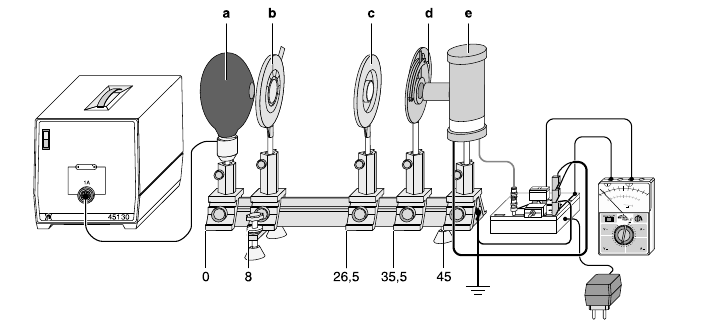
\includegraphics[width=.9\textwidth]{Figures/Planckaufbau.png}
          \caption{Versuchsaufbau auf der Optischen Bank. \textbf{a}:
              Hg-Hochdrucklampe, \textbf{b}: Irisblende,  \textbf{c}: Linse 
              f=100mm, \textbf{d}: Frequenz-Filterrad, \textbf{e}: Photozelle. 
              Positionsangaben in \textit{cm}. \cite{bib:LDDidactic}}
          \label{fig:Planckaufbau}
        \end{center}
      \end{figure}
      Nach der Jusiterung des Aufbaus ist es wichtig die Fotozelle richtig an
      zu schließen. Wir wollen zwischen Anode und Kathode ein variierbares 
      Gegenfeld haben, um die ausgelösten Elektronen auszubremsen und darüber 
      deren Energie zu bestimmen. Hierfür schließt man die Anode an den 
      negativen Ausgang eines Spannungsteilers angeschlossen und die Kathode 
      an den Postiven, welcher auf Masse gezogen wird. Ein Netzgerät mit bis 
      zu $\SI{12}{\volt}$ liegt an den Spanungsteiler an, zwischen dessen 
      Ausgängen ein Spannungsmessgerät geschaltet ist.
      
    \end{section}
    %%%%%%%%%%%%%%%%%%%%%%%%%%%%%
    
    
    
    %%%%%%%%%%%%%%%%%%%%%%%%%%%%%
    %%%%%%%%%%%%%%%%%%%%%%%%%%%%%
    %%%%%%%%%%%%%%%%%%%%%%%%%%%%%
    \begin{section}{Durchführung}
      \label{chp:Aufbau:sec:ERSTERTEIL:subsec:UNTERTEIL}
      Wir beginnen die Durchführung, indem wir das Filterrad auf den
      kurzwelligsten Filter stellen, an dem Netzgeräte die Gegenspannung hoch 
      drehen, bis kein Photostrom mehr fließt und uns aus der größe der 
      Spannung überlegen wie der Spannungsteile zusammen gestellt werden soll. 
      Wir haben aus den vorhanenden Wiederständen (zwei mal $\SI{100}{\ohm}$, 
      und je einmal $\SI{220}{\ohm}$ und $\SI{330}{\ohm}$) ein eine 
      Spannungsteilerschaltung mit einem Verhältnis von $\frac{100}{330}$ 
      gewählt. Nun sollen für die verschiedenen Filter jeweils zwei mal die 
      Kennlinien aufgenommen werden.
      %Hierzu ermittelt man zuerst den kleinst möglichen Strom, unser $I_0$ 
      Um die Kennlinie zu bestimmen beginnt man bei $U=\SI{0}{\volt}$ und
      erhöht langsam die Spannung, bis $I=\SI{0}{\ampere}$, also bis sich die 
      Werte für den Strom nicht mehr ändern. An dieser Stelle sind wir 
      zunächst jeden Filter einmal durchgegangen. Vor dem zweiten Durchgang 
      haben wir festgestellt, dass die Schutzkappe verrutscht ist, wodurch die 
      Intensität, welche die Kathode erreicht hat mit der Zeit langsam 
      abgeschwächt wurde. Um das im nächsten Durchgang zu vermeiden haben wir 
      die Schutzkappe erneut ausgerichtet und mit Klebeband fixiert. Hierdurch 
      ist es zu einer großen Intesitätsdifferenz zwischen den beide 
      aufgenommenen Kennlinien gekommen. Im Anschluss wird für die Wellenlänge 
      $\lambda = \SI{365}{\nano\meter}$ die Intesität deutlich vergrößert und 
      erneut eine Kennlinie aufgenommen.  

    \end{section}
    %%%%%%%%%%%%%%%%%%%%%%%%%%%%%
    
    
    
    %%%%%%%%%%%%%%%%%%%%%%%%%%%%%%
    %%%%%%%%%%%%%%%%%%%%%%%%%%%%%%
    %%%%%%%%%%%%%%%%%%%%%%%%%%%%%%
    \begin{section}{Auswertung des ersten Versuchstages}
      \label{chp:Photoeffekt:sec:Auswertung}
      \begin{figure}[b!]
        \begin{center}
          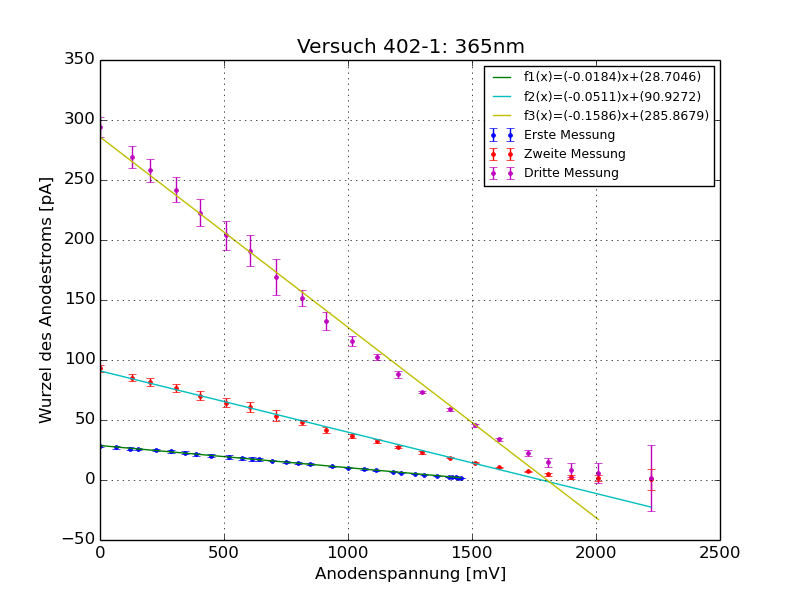
\includegraphics[width=\textwidth]{Figures/Versuch402_1_365.png}
          \caption{Messdaten für drei unterschiedliche Intensitäten.
              Wellenlänge: \SI{365}{\nano\meter}}
          \label{fig:Versuch402_1_365}
        \end{center}
      \end{figure}
      Um das Plancksche Wirkungsquantum zu bestimmen müssen bei jeder Messung
      die jeweilige Grenzspannung bestimmt werden. Diese können sehr einfach 
      aus den Graphen abgelesen werden. Die Grenzspannung findet sich für jede 
      Wellenlänge als X-Achsen Schnittpunkt, da die Grenzspannung jene ist, 
      bei der der Anodenstrom verschwindet. Die Messung der niedrigsten 
      Wellenlänge haben wir für drei unterschiedliche Intensitäten vorgenommen 
      um zu zeigen, dass die Granzspannung unabhängig der Intensität ist und 
      ausschließich durch die Wellenlänge bestimmt wird. In 
      \cref{fig:Versuch402_1_365} kann man gut erkennen, dass diese 
      Abhängigkeit tatsächlich zutrifft. In 
      \crefrange{fig:Versuch402_1_405}{fig:Versuch402_1_578} sind alle 
      Messdaten der anderen Wellenlängen ebenfalls in unterschiedlichen 
      Intensitäten dargestellt. Um aus diesen Messwerten tatsächlich das 
      Plancksche Wirkungsquantum zu bestimmen müssen die verschiedenen 
      Grenzspannungen gegen die zugehörige Frequenz der Photonen aufgetragen 
      und eine Gerade an die Messwerte angepasst werden. Aus der 
      Resultierenden Steigung lässt sich mit \cref{eq:Ekin} und der Elektronen 
      Ladung das Plancksche Wirkungsquantum berechnen. Aus unseren Messungen 
      erhalten wir eine Steigung der Grenzspannungen von 
      $\SI{3.7993e-15}{\volt\per\hertz}$. Daraus berechnet sich für unsere 
      Messungen ein Wirkungsquantum $h=\SI{6.0865e-34}{\joule\second}$. 
      
      \begin{figure}[htbp]
        \centering
        \begin{minipage}{0.48\textwidth}
          \centering
          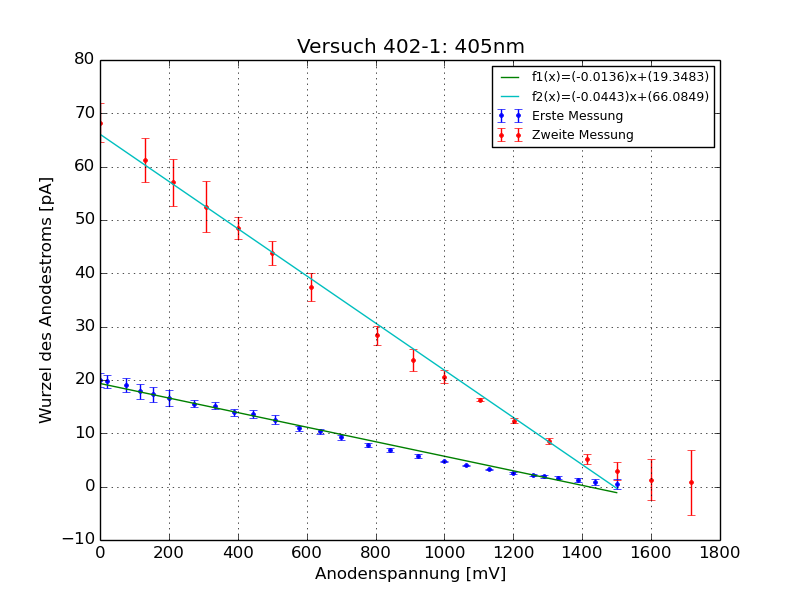
\includegraphics[width=\textwidth]{Figures/Versuch402_1_405.png}
          \caption{Messdaten für zwei unterschiedliche Intensitäten. 
              Wellenlänge: \SI{405}{\nano\meter}}
          \label{fig:Versuch402_1_405}
        \end{minipage}\quad
        \begin{minipage}{0.48\textwidth}
          \centering
          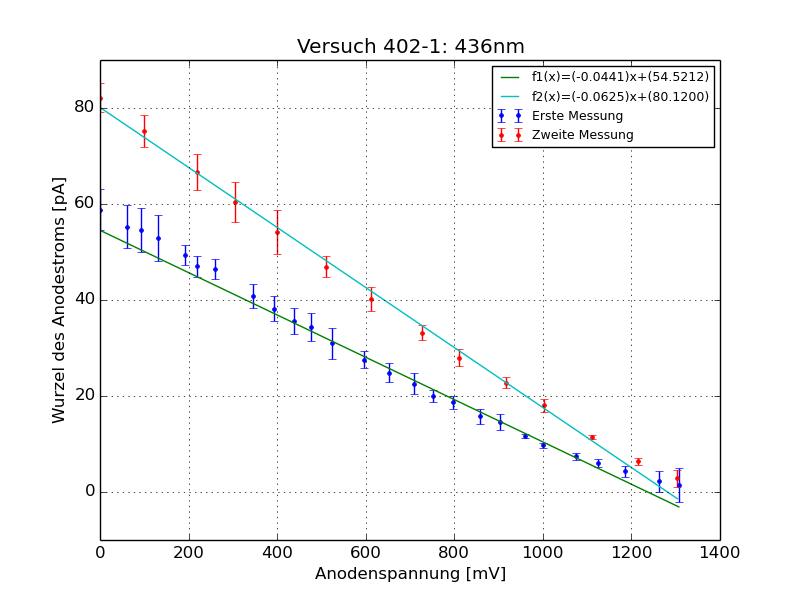
\includegraphics[width=\textwidth]{Figures/Versuch402_1_436.png}
          \caption{Messdaten für zwei unterschiedliche Intensitäten. 
              Wellenlänge: \SI{436}{\nano\meter}}
          \label{fig:Versuch402_1_436}
        \end{minipage}
        \begin{minipage}{0.48\textwidth}
          \centering
          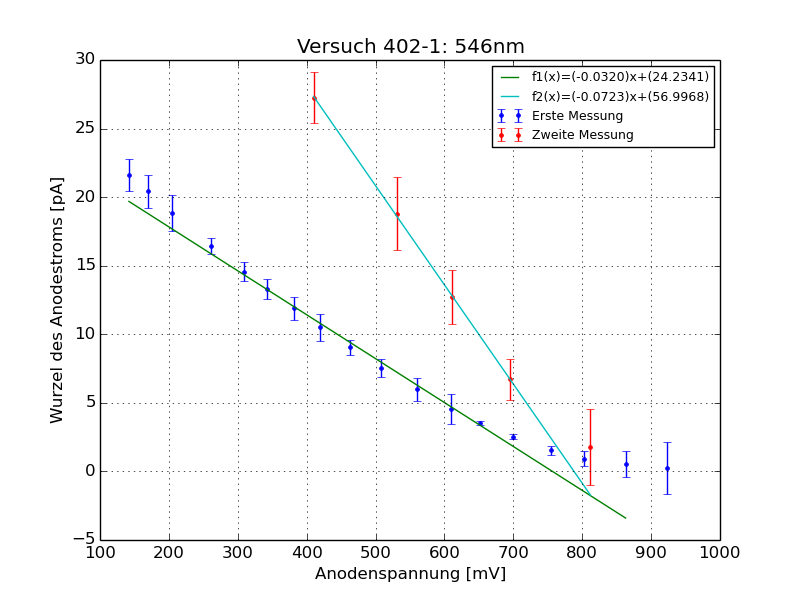
\includegraphics[width=\textwidth]{Figures/Versuch402_1_546.png}
          \caption{Messdaten für zwei unterschiedliche Intensitäten. 
              Wellenlänge: \SI{546}{\nano\meter}}
          \label{fig:Versuch402_1_546}
        \end{minipage}\quad
        \begin{minipage}{0.48\textwidth}
          \centering
          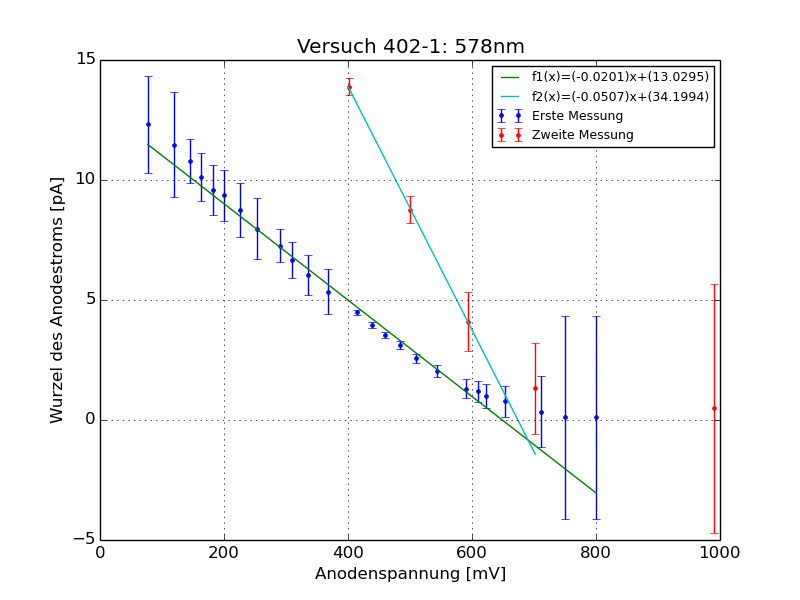
\includegraphics[width=\textwidth]{Figures/Versuch402_1_578.png}
          \caption{Messdaten für zwei unterschiedliche Intensitäten. 
              Wellenlänge: \SI{578}{\nano\meter}}
          \label{fig:Versuch402_1_578}
        \end{minipage}
      \end{figure}
      
      \begin{figure}[htbp]
        \begin{center}
          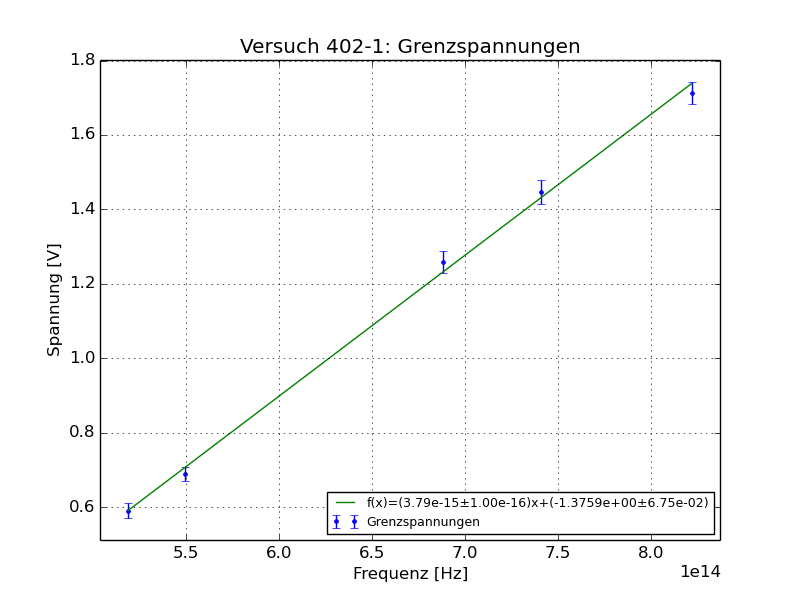
\includegraphics[width=.8\textwidth]
          {Figures/Versuch402_1_PlanckschesWirkungsquant.png}
          \caption{Graphische Darstellung aller Grenzspannungen zur Bestimmung
              des Planckschen Wirkungsquantum.}
          \label{fig:Versuch402_1_PlanckschesWirkungsquant}
        \end{center}
      \end{figure}
      
    \end{section}
    %%%%%%%%%%%%%%%%%%%%%%%%%%%%%%
    
    
    
    %%%%%%%%%%%%%%%%%%%%%%%%%%%%%%
    %%%%%%%%%%%%%%%%%%%%%%%%%%%%%%
    %%%%%%%%%%%%%%%%%%%%%%%%%%%%%%
    \begin{section}{Fazit - Photoeffekt}
      \label{chp:Photoeffekt:sec:Fazit}
      Zusammenfassend können wir nicht sagen, dass unsere Messung eine
      tatsächlich genaue Bestimmung des Planckschen Wirkungsquantum lieferte da 
      die Abweichung zum Literaturwert von 
      $h_{Lit}=\SI{6.62607e-34}{\joule\second}$ leider nicht zu leugnen sind.
      
      \todo[inline]{Am besten noch etwas mehr schreiben}
      
    \end{section}
    %%%%%%%%%%%%%%%%%%%%%%%%%%%%%%
    
  \end{chapter}
  %%%%%%%%%%%%%%%%%%%%
  
  
  
  %%%%%%%%%%%%%%%%%%%%
  %%%%%%%%%%%%%%%%%%%%
  %%%%%%%%%%%%%%%%%%%%
  \begin{chapter}{Zweiter Versuchsteil - Balmer-Serie}
    \label{chp:Balmer}
  
  
    %%%%%%%%%%%%%%%%%%%%%%%%%%%%%%
    %%%%%%%%%%%%%%%%%%%%%%%%%%%%%%
    %%%%%%%%%%%%%%%%%%%%%%%%%%%%%%
    \begin{section}{Aufbau}
      \label{chp:Balmer:sec:Aufbau}
      \todo[inline]{skizze}
      Ziel dieses Versuchsteils ist es, dass Spektrum einer 
      Wasserstoff-Deuterium-Lampe, die so genannte Balmerserie, zu bestimmen.
      Hierzu nutzen wir ein Rfelexionsgitter, welches zwischen zwei gewinkleten
      Armen einer optischen Bank steht. Der Winkel zwischen beiden Armen kann 
      abgelesen werden. Zu Beginn stehen an dem einen Ende der optischen Bank 
      eine Hg Lampe und am anderen ein Okular mit Strichskala, um die 
      Gitterkonstante zu bestimmen. Im Verlauf des Versuchs wir zuerst die 
      Lampe gegen die Wasserstoff-Deuterium-Lampe und später das Okular gegen 
      einen CCD-Kamera ausgetauscht. Die gesammt Anordnung ist, wie auch auf 
      dem Bilder zu sehen, Balmer-Lampe, Linse mit einer Brennweite von 
      $f=\SI{50}{\milli\meter}$, ein verstellbarer Spalt, ein 
      Projektionsojektiv mit $f=\SI{150}{\milli\meter}$, das 
      Refelxionsgitter,eine weitere Linse mit $f=\SI{300}{\milli\meter}$ und 
      zu guter letztdas Okular, beziehungsweise die CCD-Kamera.

    \end{section}
    %%%%%%%%%%%%%%%%%%%%%%%%%%%%%%
    
    
    
    %%%%%%%%%%%%%%%%%%%%%%%%%%%%%%
    %%%%%%%%%%%%%%%%%%%%%%%%%%%%%%
    %%%%%%%%%%%%%%%%%%%%%%%%%%%%%%
    \begin{section}{Justierung und Durchführung}
      \label{chp:Balmer:sec:JusitierungDurchfuehrung}
      
      
      
      %%%%%%%%%%%%%%%%%%%%%%%%%%%%%%%%%%%%%%%%
      %%%%%%%%%%%%%%%%%%%%%%%%%%%%%%%%%%%%%%%%
      %%%%%%%%%%%%%%%%%%%%%%%%%%%%%%%%%%%%%%%%
      \begin{subsection}{Justierung}
        \label{chp:Balmer:sec:JusitierungDurchfuehrung:subsec:Justierung}
        Zunächst ist der Anfangsaufbau mit der Hg Lampe zu Justieren. Nach
        einsetzen der Lampe wird die erste Linse ($f=\SI{50}{\milli\meter}$) 
        so eingesetzt, das sie die Lichtquelle auf die schrägen Flanken des 
        senkrecht stehenden Splates abbildet. Als nächstes wird das Objektiv 
        eingesetzt und mit Hilfe der Autokollimation justiert. Das lässt sich 
        realisieren, indem man das Gitter so dreht, dass die Reflektion erneut 
        durch das Objektiv fällt und somit den Spalt neben den Spalt abbildet. 
        Wenn man diese Abbildung des Splates nun scharf stellt, ist diese nach 
        dem Objektiv auf Unendlich fokussiert. Nun legen wir die Abbildung des 
        Spaltes über dem Spalt und stellen den Winkel zwischen den Armen der 
        optischen Bänke auf $\alpha-\beta = \SI{30}{\degree}$. Dieser Winkel 
        wird von uns den ganzen Versuch über nicht geändert. Am Ende des 
        zweiten Armses wird das Okular so montiert, dass die Skala gut 
        abzulesen ist. Um die verschiedenen Spektrallinien auf die Skala 
        scharf ab zu bilden stellen man die letzte Linse in den Strahlengang 
        und verschiebt diese je nach bedarf. So entsteht ein 
        Beobachtungsteleskop.

      \end{subsection}
      %%%%%%%%%%%%%%%%%%%%%%%%%%%%%%%%%%%%%%%%
      
      
      
      %%%%%%%%%%%%%%%%%%%%%%%%%%%%%%%%%%%%%%%%
      %%%%%%%%%%%%%%%%%%%%%%%%%%%%%%%%%%%%%%%%
      %%%%%%%%%%%%%%%%%%%%%%%%%%%%%%%%%%%%%%%%
      \begin{subsection}{Bestimmung der Gitterkonstante}
        \label{chp:Balmer:sec:JusitierungDurchfuehrung:subsec:Gitter}
        Um Gitterkonstante zu bestimmen nehmen wir die Hg Lampe. Diese benutzen
        wir, da sie eine hohe Intesität hat, wodurch die Spektrallinien gut 
        sichtbar sind. Außerdem haben kennen wir deren Wellenlängen und können 
        so diese den beobachteten Wellenlängen identifizieren um die 
        Gitterkonstante zu bestimmen. Wir drehen an der Gittersäule so, um die 
        ersten Linien im Okular sichtabr zu machen. Nun stellen wir mit Hilfe 
        der $f=\SI{300}{\milli\meter}$ Linse die Linien scharf und notieren 
        uns die Farbe und den Gitterwinkel $\omega_G$. So gehen wir vor bis 
        wir alle sichtbaren Linien notiert haben. Durch den vergleich mit den 
        gegebenen Wellenlängen für Spektrallinien lassen sich so den Winkel 
        Wellenlängen zu ordnen.
        
        \todo[inline]{Tabelle}

      \end{subsection}
      %%%%%%%%%%%%%%%%%%%%%%%%%%%%%%%%%%%%%%%%
      
      %%%%%%%%%%%%%%%%%%%%%%%%%%%%%%%%%%%%%%%%
      %%%%%%%%%%%%%%%%%%%%%%%%%%%%%%%%%%%%%%%%
      %%%%%%%%%%%%%%%%%%%%%%%%%%%%%%%%%%%%%%%%
      \begin{subsection}{Untersuchung der Balmer-Linie mit einem Okular}
        \label{chp:Balmer:sec:JusitierungDurchfuehrung:subsec:Okular}
        Als nächstes tauschen wir die Hg Lampe durch eine Balmer-Lampe und
        überprüfen die Justierung. Dann suchen wir durch drehen der Gittersäule 
        erneut die erste Linie und notieren uns die Farbe, den Winkel und die 
        Breite der Linien $d$, welche den Abstand der Aufspaltung der 
        Linienbreite representiert. Hierfür ist besonders wichtig die Linen 
        auf die Skala scharf zu stellen. Für die anderen Linien wiederholen 
        wir dieses Vorgehen.
          
        \todo[inline]{tabelle}

      \end{subsection}
      %%%%%%%%%%%%%%%%%%%%%%%%%%%%%%%%%%%%%%%%
      
      %%%%%%%%%%%%%%%%%%%%%%%%%%%%%%%%%%%%%%%%
      %%%%%%%%%%%%%%%%%%%%%%%%%%%%%%%%%%%%%%%%
      %%%%%%%%%%%%%%%%%%%%%%%%%%%%%%%%%%%%%%%%
      \begin{subsection}{Untersuchung der Balmerlinie mit der CCD-Kamera}
        \label{chp:Balmer:sec:JusitierungDurchfuehrung:subsec:CCD}
        Für den nächsten Versuchteil wird das Okular durch die CCD-Kamera 
        ersetzt. Dabei muss dadrauf geachtet werden, dass CCD-Zeile beleuchtet 
        wird. Die Kamera wird an den PC angeschlossen und mit Strom versorgt. 
        Auf dem PC öffnet man Das Programm VideoCom und wählt die 
        Einstellungen aus der Versuchsanleitung. Wir wollen die 
        Isotropieaufspaltung messen, also suchen wir nach Ausschlägen, indem 
        wir mit der Gittersäule die Winkel ansteuern, die wir zuvor ermittelt 
        haben. Sobald auf dem Monitor einer dieser Ausschläge erscheint, 
        versuchen wir durch Vergrößerung des Abschnittes, Mittelwertbildung 
        der Intesität und verschieben der letzten Linse zwei scharfe getrennte 
        Spitzen oder Überlagerungen zu erhalten. Aus den so aufgenommenen 
        Messdaten lässt sich die Linienverbreiterung bestimmen.

        \todo[inline]{messwerte?}

      \end{subsection}
      %%%%%%%%%%%%%%%%%%%%%%%%%%%%%%%%%%%%%%%%

    \end{section}
    %%%%%%%%%%%%%%%%%%%%%%%%%%%%%%
    
    
    
    %%%%%%%%%%%%%%%%%%%%%%%%%%%%%%
    %%%%%%%%%%%%%%%%%%%%%%%%%%%%%%
    %%%%%%%%%%%%%%%%%%%%%%%%%%%%%%
    \begin{section}{Auswertung}
      \label{chp:Balmer:sec:Auswertung}
      
    \end{section}
    %%%%%%%%%%%%%%%%%%%%%%%%%%%%%%
    
    
    
    %%%%%%%%%%%%%%%%%%%%%%%%%%%%%%
    %%%%%%%%%%%%%%%%%%%%%%%%%%%%%%
    %%%%%%%%%%%%%%%%%%%%%%%%%%%%%%
    \begin{section}{Fazit}
      \label{chp:Balmer:sec:Fazit}
      
    \end{section}
    %%%%%%%%%%%%%%%%%%%%%%%%%%%%%%
    
  \end{chapter}
  %%%%%%%%%%%%%%%%%%%%
  
  
  %%%%%%%%%%%%%%%%%%%%
  %%%%%%%%%%%%%%%%%%%%
  %%%%%%%%%%%%%%%%%%%%
  \begin{appendix}
    \label{Anhang}
    
    
    
    %%%%%%%%%%%%%%%%%%%%%%%%%%%%%%
    %%%%%%%%%%%%%%%%%%%%%%%%%%%%%%
    %%%%%%%%%%%%%%%%%%%%%%%%%%%%%%
    \begin{chapter}{ERSTER TEIL}
      \label{Anhang:chp:ERSTERTEIL}
      
      
      
      %%%%%%%%%%%%%%%%%%%%%%%%%%%%%%%%%%%%%%%%
      %%%%%%%%%%%%%%%%%%%%%%%%%%%%%%%%%%%%%%%%
      %%%%%%%%%%%%%%%%%%%%%%%%%%%%%%%%%%%%%%%%
      \begin{section}{ERSTER UNTERTEIL}
        \label{Anhang:chp:ERSTERTEIL:sec:UNTERTEIL}
       
       
       
      \end{section}
      %%%%%%%%%%%%%%%%%%%%%%%%%%%%%%%%%%%%%%%%
      
      
    \end{chapter}
    %%%%%%%%%%%%%%%%%%%%%%%%%%%%%%
    
  \end{appendix}
  %%%%%%%%%%%%%%%%%%%%
  
  
  
  %%%%%%%%%%%%%%%%%%%%
  %%%%%%%%%%%%%%%%%%%%
  %%%%%%%%%%%%%%%%%%%%
  \begin{thebibliography}{99}
    \scriptsize
    \bibitem{bib:PhotozelleAufbau}\url{http://www.leifiphysik.de/sites/
        default/files/medien/Kennlinie_einer_Fotozelle_Bild_2.gif}
    \bibitem{bib:Photoeffekt}\url{http://web-docs.gsi.de/~wolle/TELEKOLLEG/
        ATOM/IMAGES/photoeffekt1.gif}
    \bibitem{bib:BalmerserieEmissionAbsorption}\url{http://scienceblogs.de/
        primaklima/wp-content/blogs.dir/29/files/2012/06/
        i-86621a49589f7ddc22387aa065cef996-Balmerserie.jpg}
    \bibitem{bib:BohrschesAtommodellSerien}\url{http://www.systemdesign.ch/
        images/4/4e/BohrschesAtommodellSerien.jpg}
    \bibitem{bib:LDDidactic} \url{TODO}
    
  \end{thebibliography}
  %%%%%%%%%%%%%%%%%%%%
  
\end{document}
%%%%%%%%%%
